\section{Defining the MAL effect in the UD collection}\label{metrics}

We call $\lambda$MAL(L) the function that mapst MAL$_n$(L) to each $n$. It has been shown by \citet{altmann1980prolegomena} that a function such as $\lambda$MAL(L) should follow a power law. In other words, MAL$_n$(L) is expected to be more or less proportional to $n^{-\beta}$ where $\beta$ is a positive value (generally smaller than 1), which we call the MAL effect for L. 
Note that if MAL$_n$(L) $\approx n^{-\beta}$, then log(MAL$_n$(L)) $\approx -\beta$log($n$). In other word, $-\beta$ is the slope of the regression line of the log-log representation of $\lambda$MAL(L). The greater is $\beta$, the quicker is the decrease, the stronger is the MAL effect. Figure \ref{fig:German} gives the value of $\beta$ (1.171) as well as the coefficient $R^2$ (0.892), which shows that $\lambda$MAL(German) is close to a power law and that MAL is verified for German.

\begin{figure}[!ht]
\begin{center}
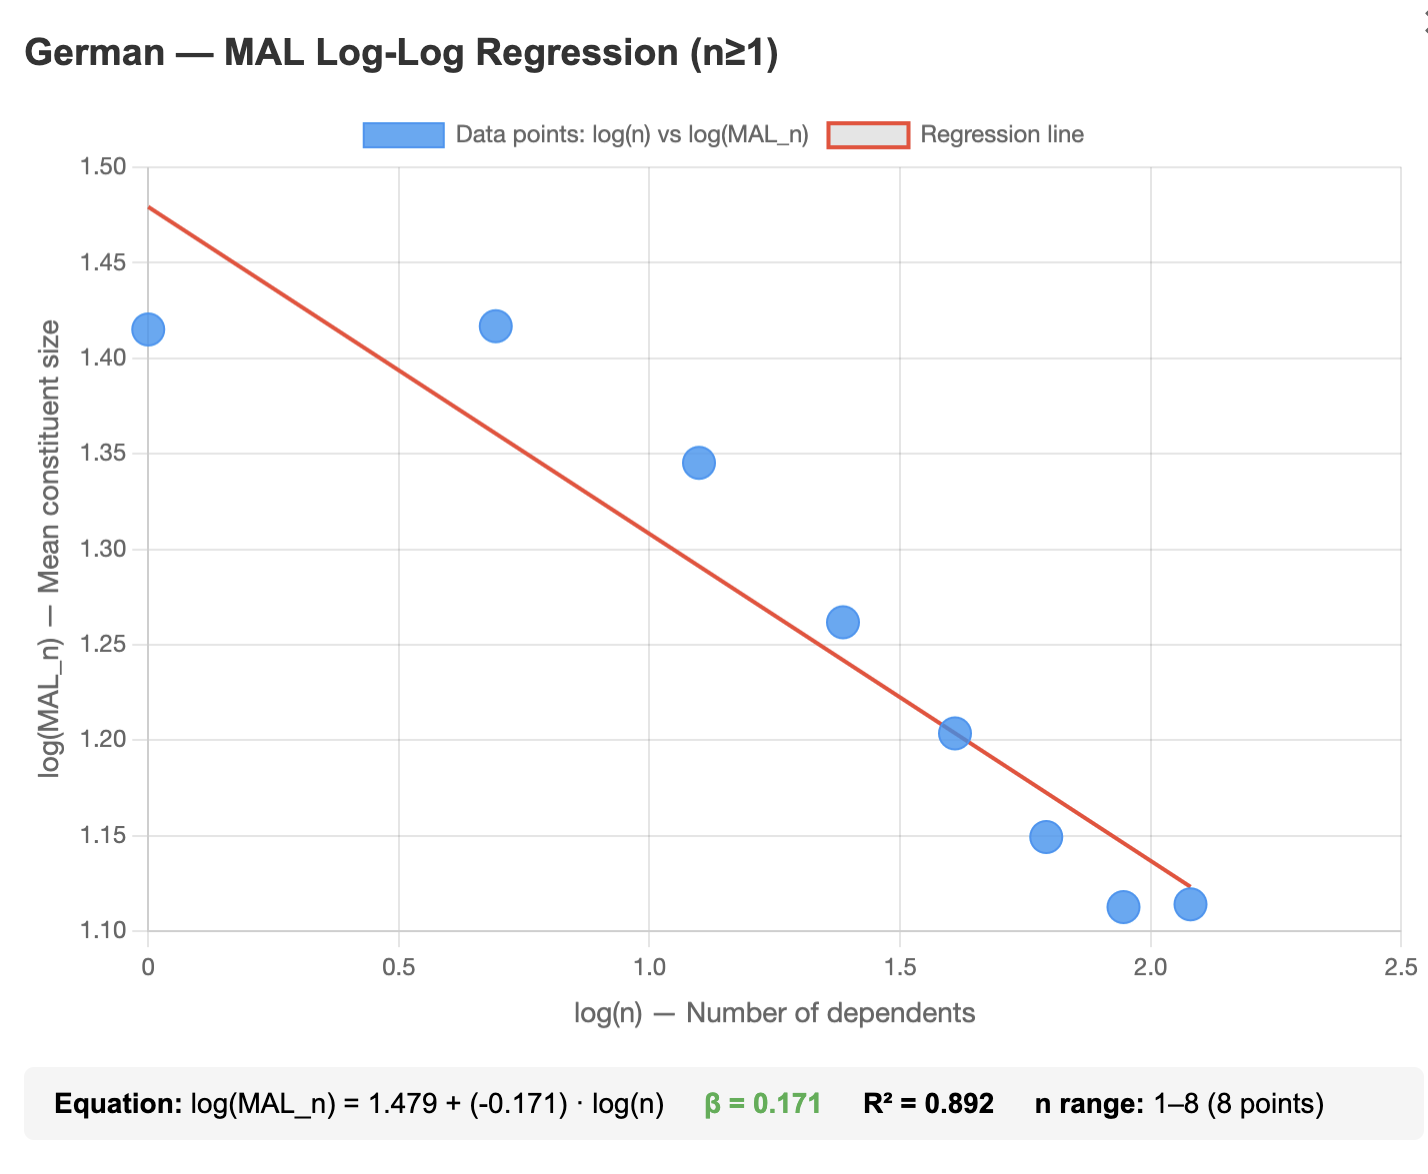
\includegraphics[width=\columnwidth]{latex/German.png}
\caption{$\lambda$MAL(German).}
\label{fig:German}
\end{center}
\end{figure}

%There are also languages that do not clearly follow a power law. This is the case of OldEast Slavic which not only has an Anti MAL effect (the mean length of the constituents increase with the number of constituents) but on top of that the Anti MAL effect increases with the number of constituents (Figure \ref{fig:OldEastSlavic}

%\begin{figure}[!ht]
%\begin{center}
%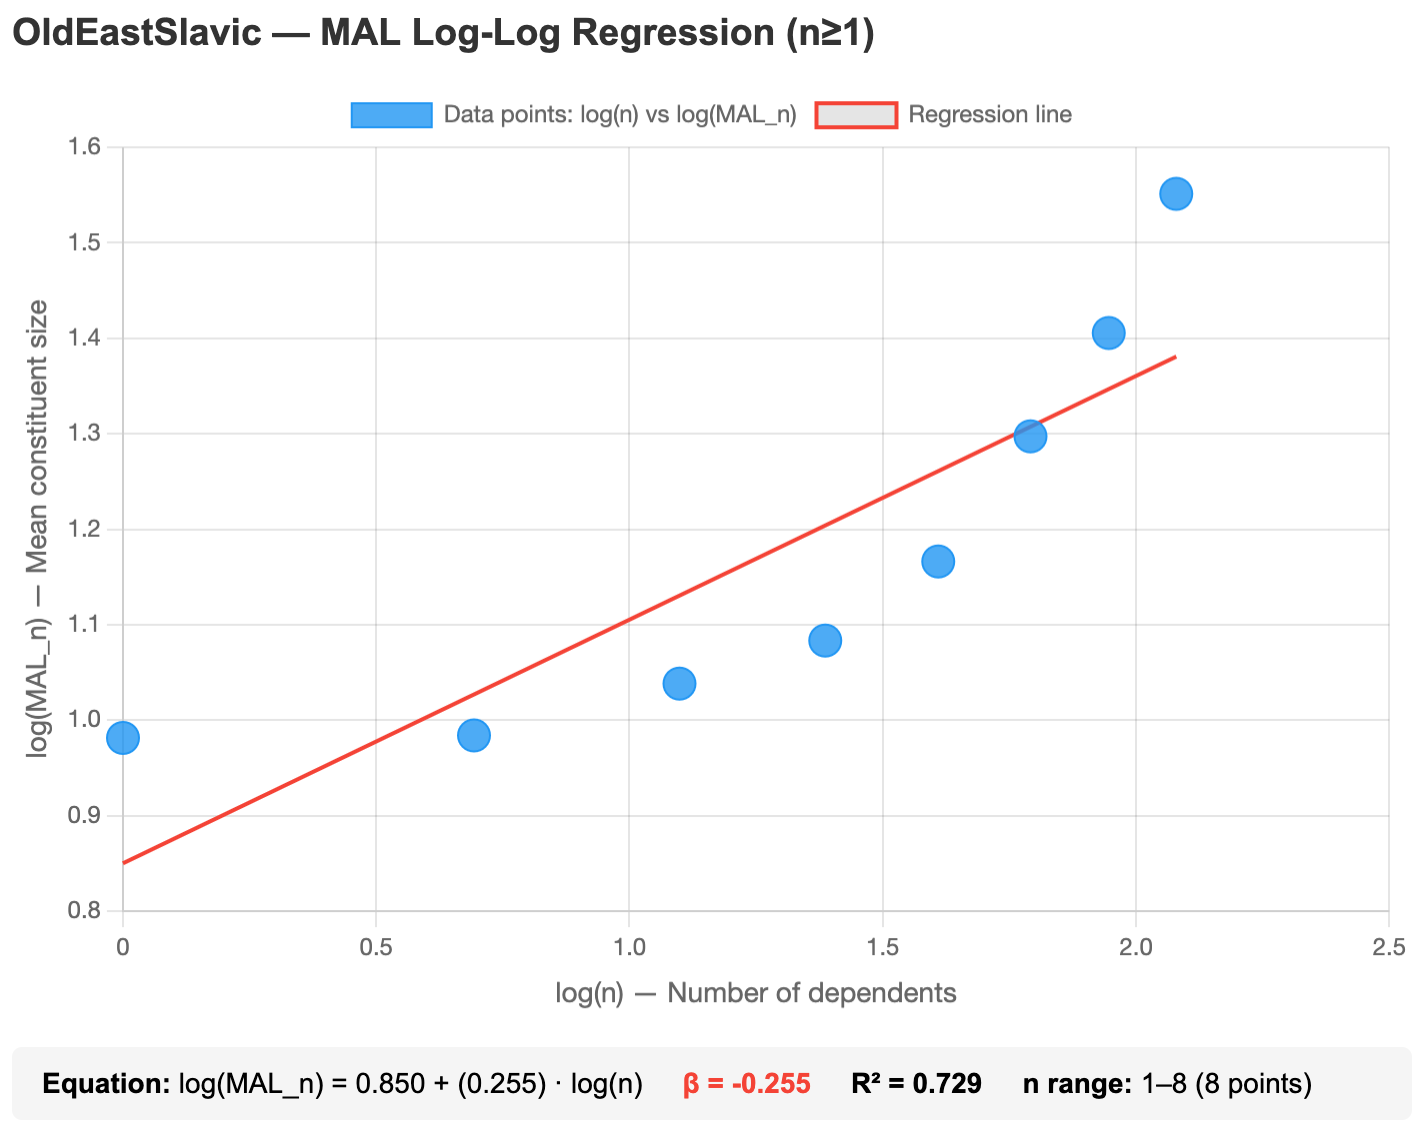
\includegraphics[width=\columnwidth]{latex/OldEastSlavic.png}
%\caption{$\lambda$MAL(OldEastSlavic).}
%\label{fig:OldEastSlavic}
%\end{center}
%\end{figure}

\citet{tanaka2021menzerath} showed that, on her data, the values for $n$ = 1 and $n$ = 2 may not be aligned and she took onto account only the values for $n\geq$ 3 for computing $\beta$. We think that the problem was was partly due to the fact that her data were not filtered.

We call $\beta$($j\rightarrow k$) the slope of $\lambda$MAL for $j\leq n \leq k$. If $k = j+1$, $\beta$($j\rightarrow k$) is just the slope between the point (log(MAL$_j$),log($j$)) and (log(MAL$_k$),log($k$)).
In the figure \ref{fig:1vs2}, we compare the $\beta$(1$\rightarrow$2) with $\beta$(2$\rightarrow\infty$). The important dispersion suggests that the value for MAL$_1$ is effectively poorly aligned with the other values. The case where MAL$_1$ is aligned are the point on the diagonal $y=x$.

\begin{figure*}[ht]
\begin{center}
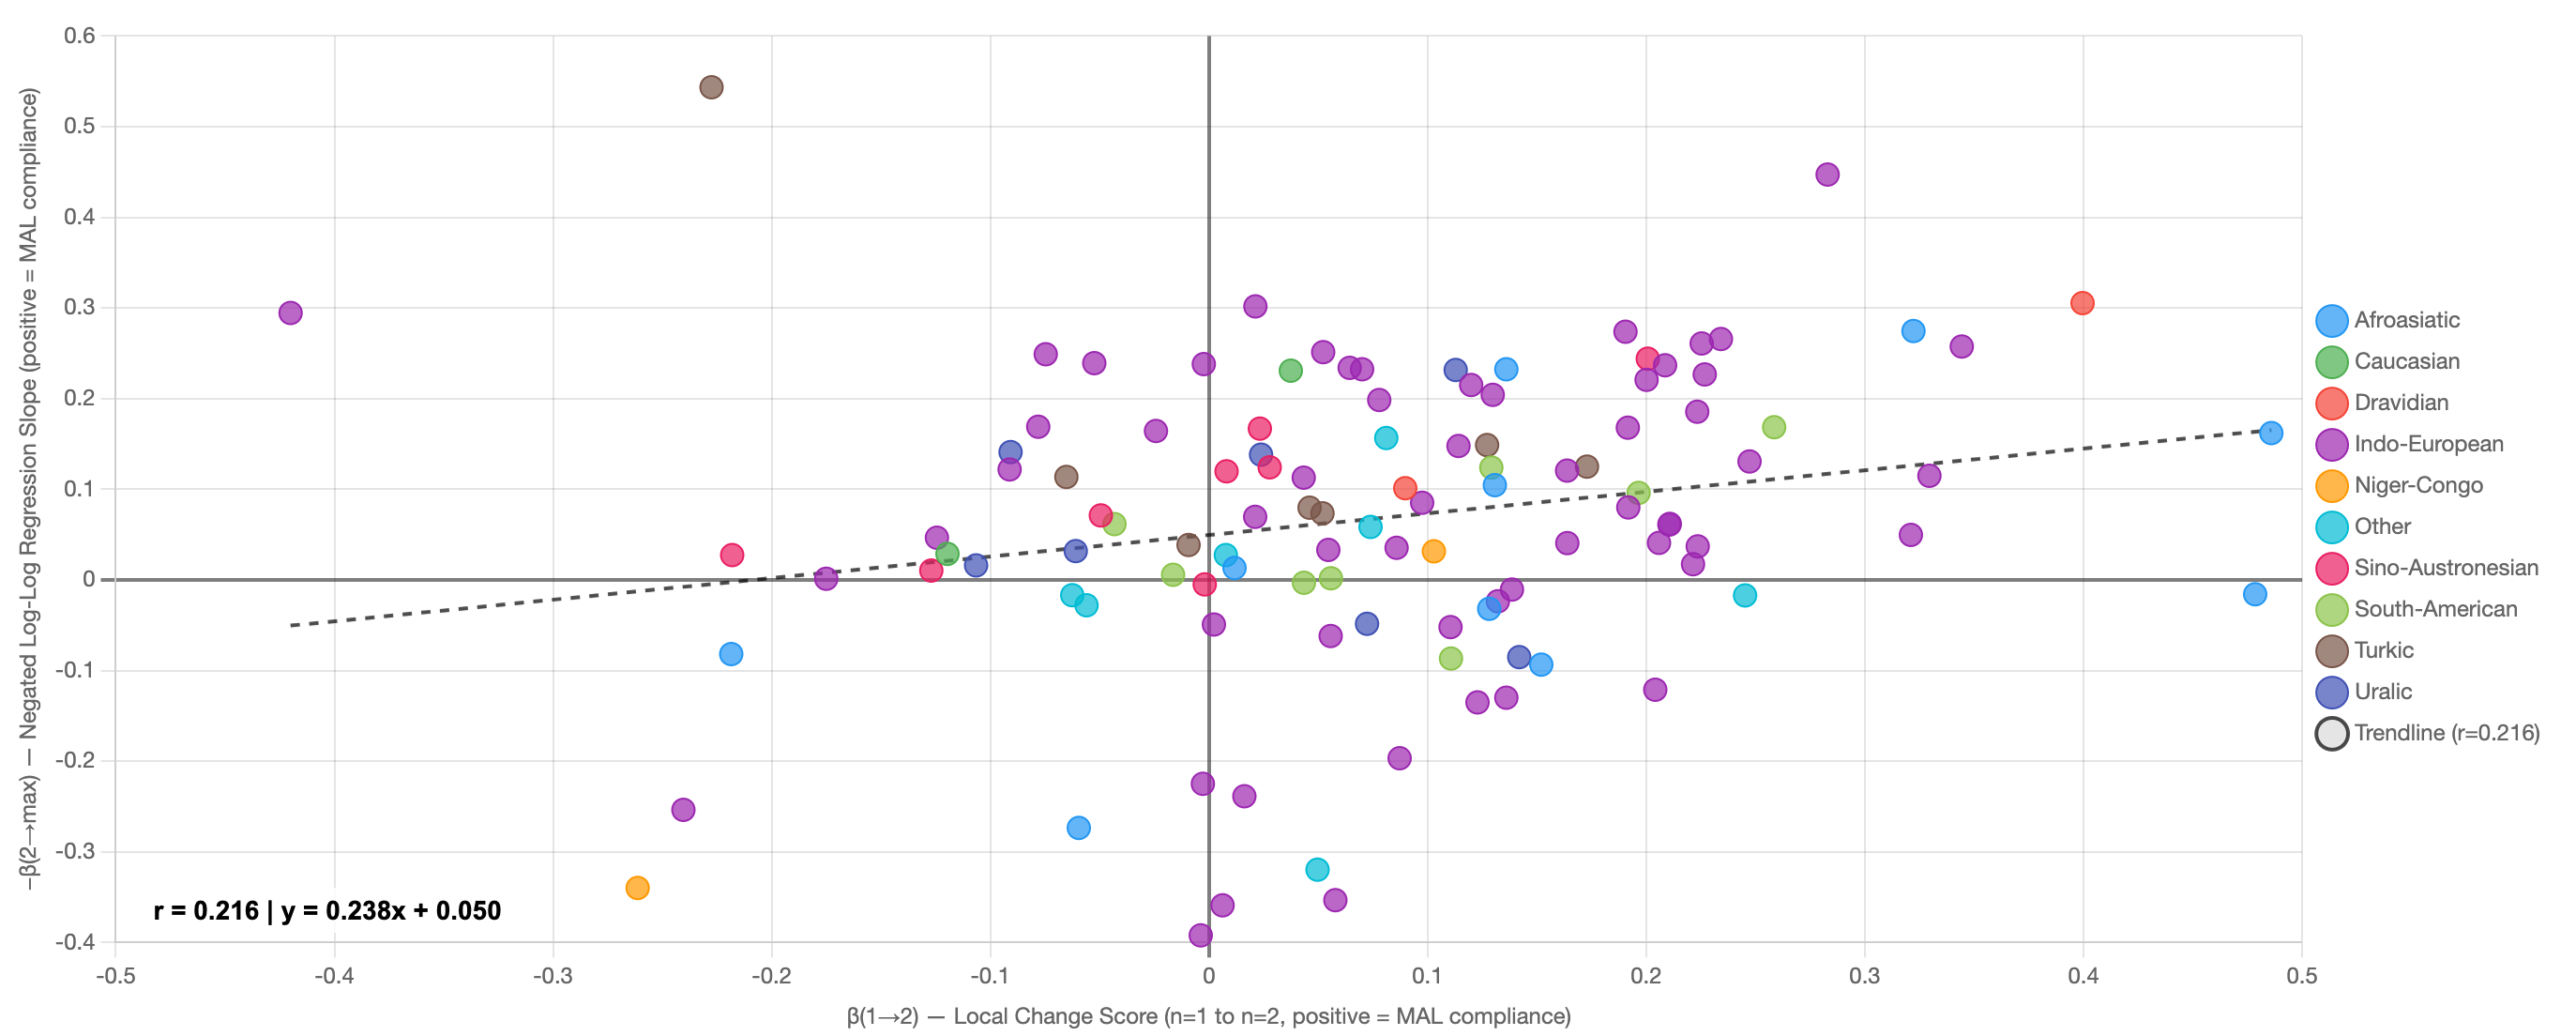
\includegraphics[width=\textwidth]{latex/1vs2.png}
\caption{$\beta$(1$\rightarrow$2) vs $\beta$(2$\rightarrow \infty$)}
\label{fig:1vs2}
\end{center}
\end{figure*}

Nevertheless we observe that the values of MAL$_1$ can be sometimes under the regression line for $n\geq 2$ (as it is the case for German, Fig. \ref{fig:German} and sometimes above (see Czech, Fig. \ref{fig:Czech}, or Arabic, Fig. \ref{fig:Arabic}).

\begin{figure}[!ht]
\begin{center}
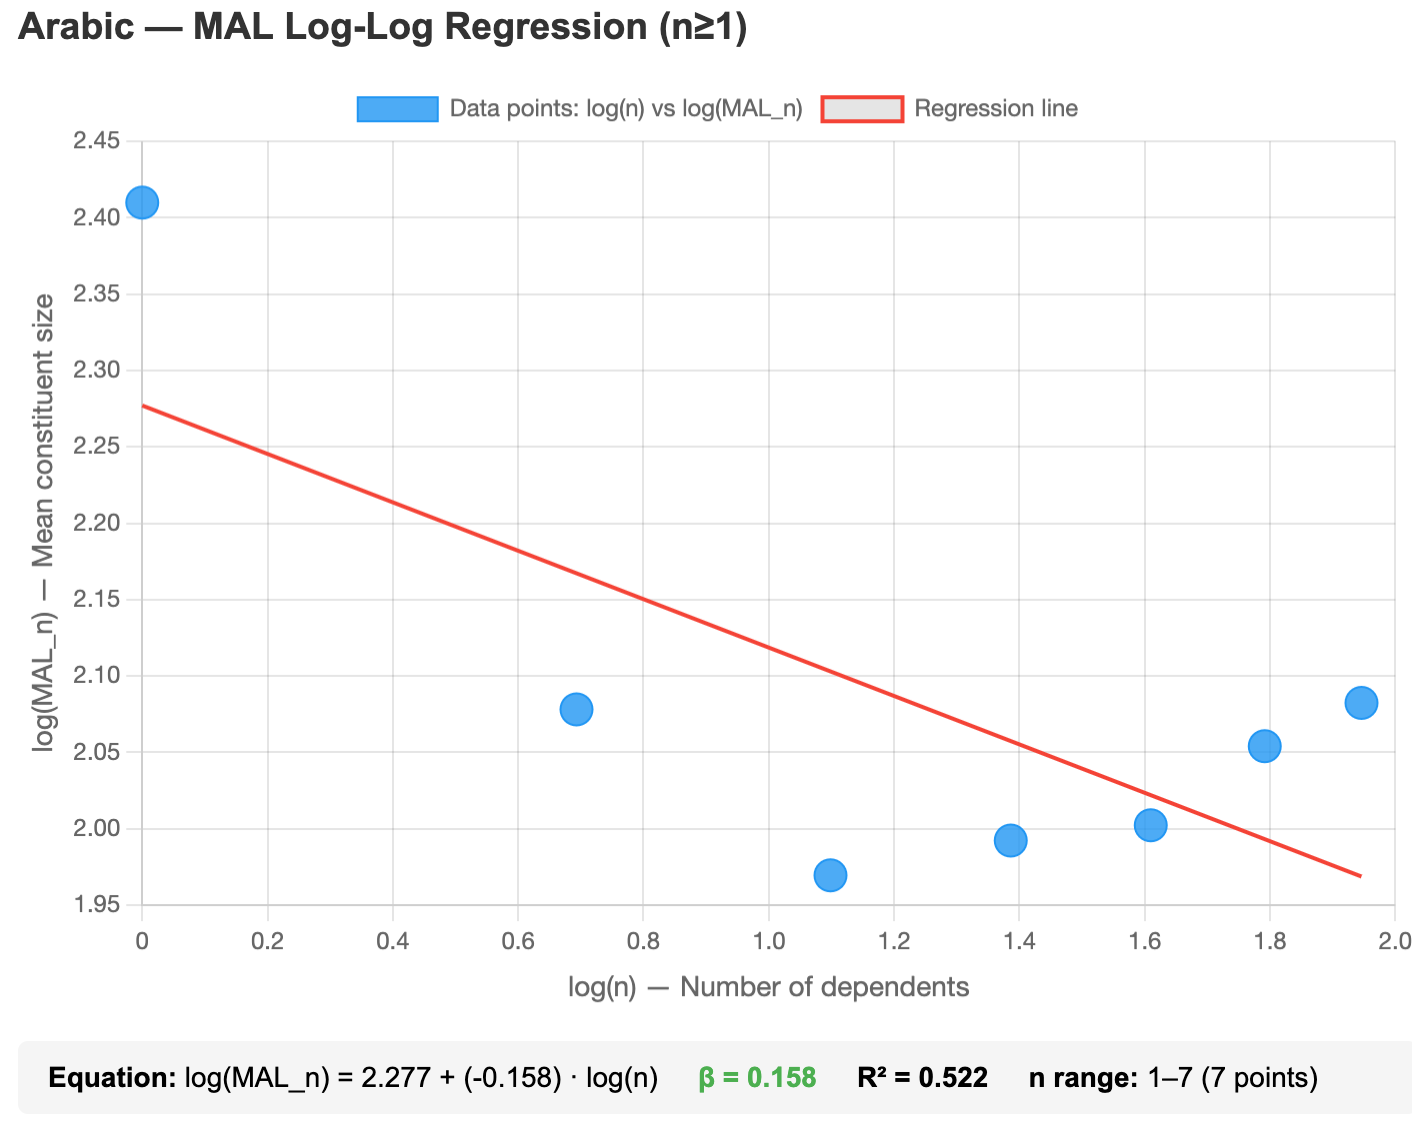
\includegraphics[width=\columnwidth]{latex/Arabic.png}
\caption{$\lambda$MAL(Arabic).}
\label{fig:Arabic}
\end{center}
\end{figure}

\begin{figure}[!ht]
\begin{center}
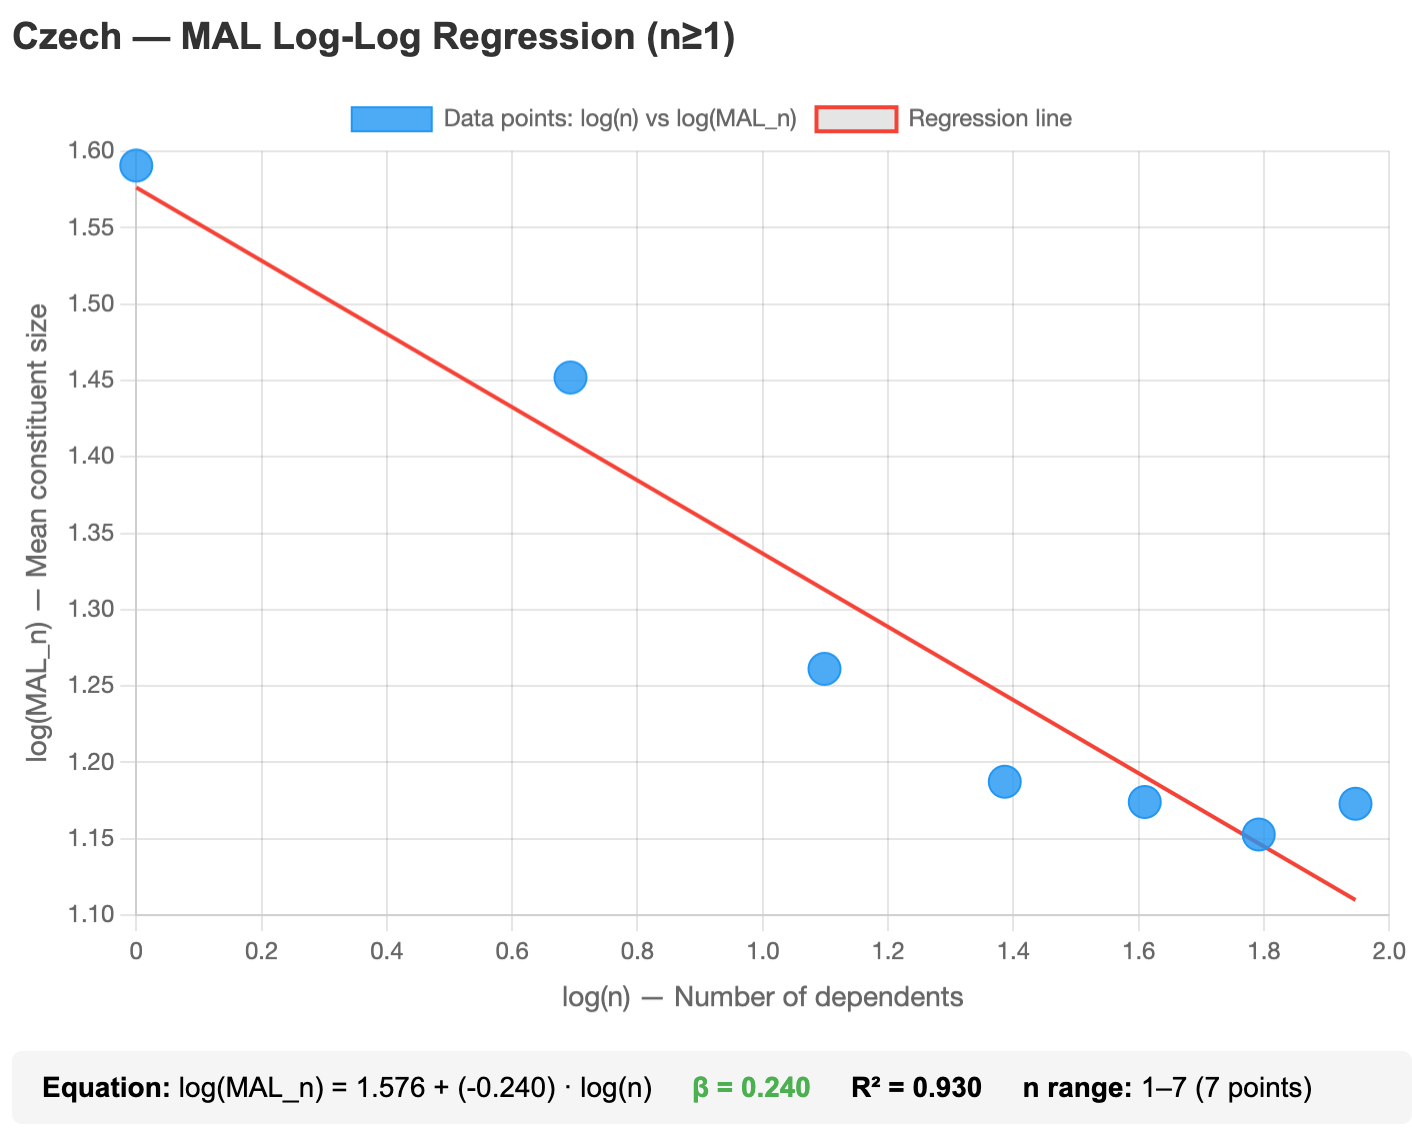
\includegraphics[width=\columnwidth]{latex/Czech.png}
\caption{$\lambda$MAL(Czech).}
\label{fig:Czech}
\end{center}
\end{figure}

We then decide to take $\beta$(1$\rightarrow\infty$) as the metric to evaluate the MAL effect. We also do that because, due to the filter and the fact that many treebanks are quite small, we do not have values of MAL$_n$ for $n\geq 4$. And it is even more problematic when we look at LMAL$_n$ and RMAL$_n$. 

 We nevertheless must mention an additional problem with $n$ = 1. While the number of configurations with $n$ constituents decrease for n $geq 2$ only 20 of the 131 languages that have at least 100 configurations for $n$ = 2 and 3 have more data $n$ = 1 than for $n$ = 2. Among them, 12 language have less that 100 configurations with one constituent ($n$ = 1) and we must take $\beta$(2$\rightarrow\infty$) to evaluate the MAL effect.
 
There are 131 languages in our sample for which we have calculated a value for $\beta$(1$\rightarrow\infty$). We identify three types of behavior in our sample and givent that our values of $\beta$(1$\rightarrow\infty$) are mainly comprised between $-0.3$ and $0.3$, we devide them into the three categories following categories:\footnote{For $\lamba$MAL, no $\beta$(1$\rightarrow\infty$) are lesser than $-0.3$ and only 9 languages have a $\beta$(1$\rightarrow\infty$) greater than $0.3$. Almost same thing for $\lamba$LMAL. For $\lamba$RMAL, 48 languages have a value greater than $0.3$!} 

\begin{itemize}
    \item Language L with $\beta$(1$\rightarrow\infty$) $\geq 0.1$ is considered to have a MAL effect;
    \item Language L with $\beta$(1$\rightarrow\infty$) $\leq -0.1$ is considered to have an Anti MAL effect.
    \item Language L with $-0.1\leq$ $\beta$(1$\rightarrow\infty$) $\leq 0.1$ is considered to be in the grey zone;
\end{itemize}

The majority of languages of our sample (that is, 62 languages which make 47\% of the 131 languages) fall into the first category, that is they show a MAL effect. But there are also a smaller number of languages (10 languages,),showing an Anti MAL effect. The remaining languages are in the gray zone (45\% of languages). 

One of the languages that do not follow a power law is OldEast Slavic, which not only has an Anti MAL effect (that is, the mean length of the constituents increase with the number of constituents), but on top of that the anti MAL effect increases with the number of constituents (Figure \ref{fig:OldEastSlavic}

\begin{figure}[!ht]
\begin{center}
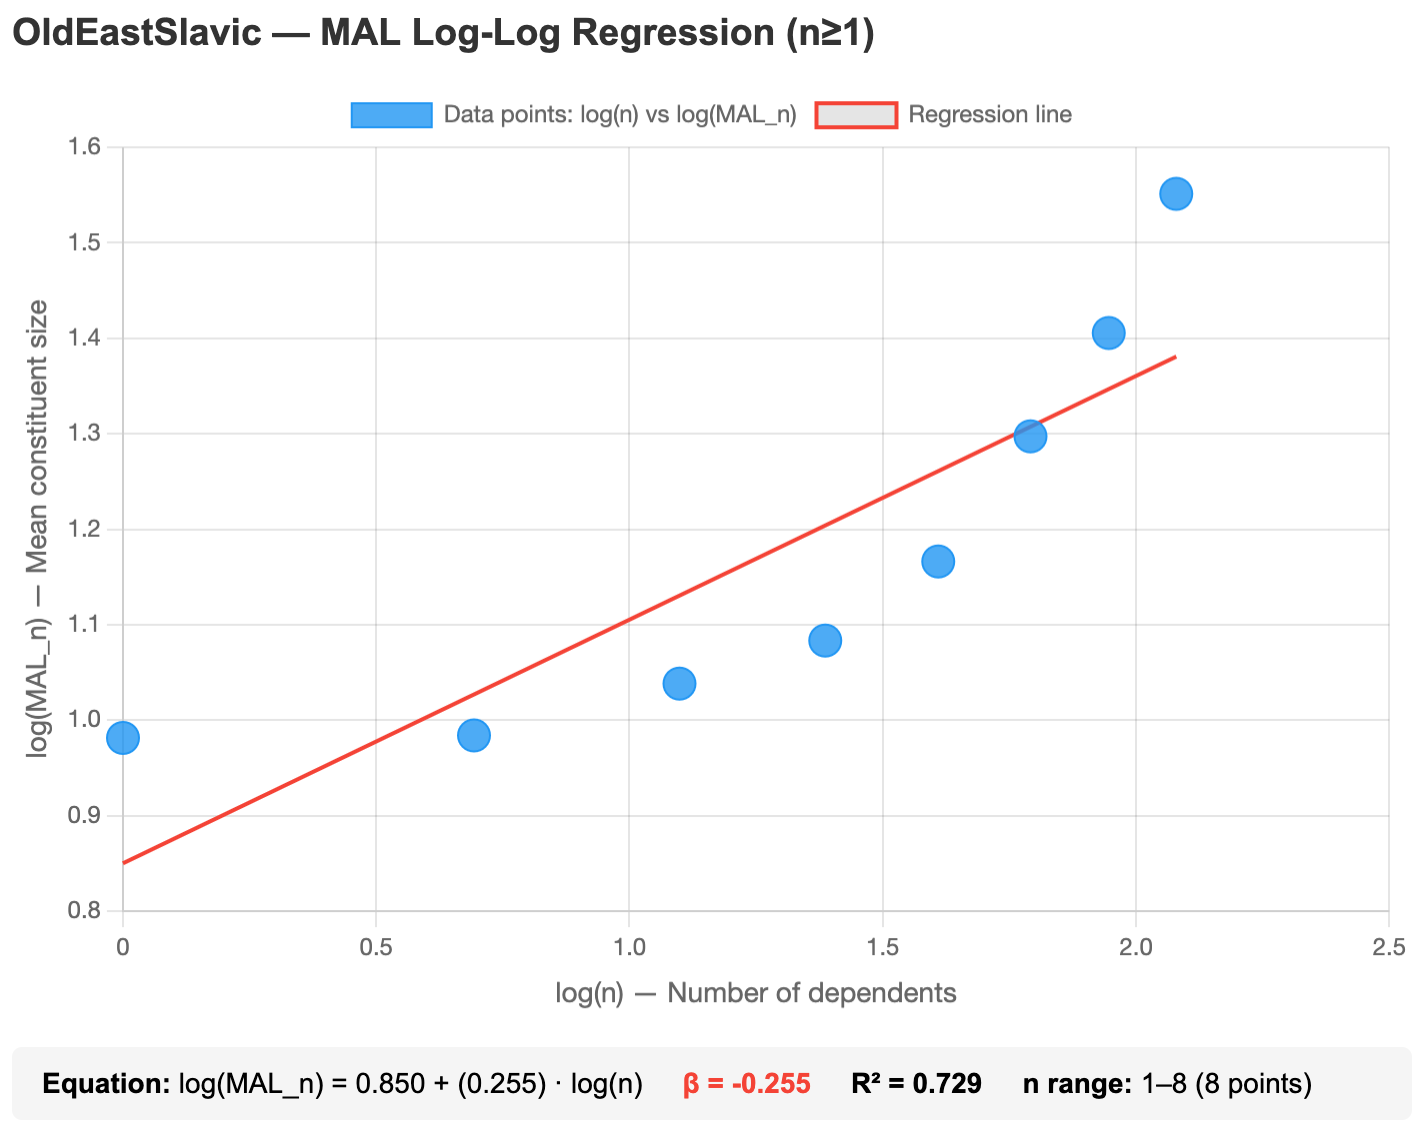
\includegraphics[width=\columnwidth]{latex/OldEastSlavic.png}
\caption{$\lambda$MAL(OldEastSlavic).}
\label{fig:OldEastSlavic}
\end{center}
\end{figure}
